% ============================================================
%  \subsection{API Design}
%  aBridgeAI — Capstone Report (main body summary)
%  Full endpoint catalogue is documented in Appendix \ref{appendix:api-design}.
% ============================================================

\subsection{API Design}

% ─────────────────────────────────────────────
\subsubsection{Architecture \& Design Philosophy}
% ─────────────────────────────────────────────

The aBridgeAI backend is a Python \textbf{FastAPI} service exposing a versioned RESTful API at the base path \path|/api/v1|. It serves as the single data contract between the Vite SPA and the server. The API surface is composed by a single \path|create_app()| factory that mounts every per-feature router under the shared \path|API_V1_PREFIX|; routers themselves carry their own per-feature prefix (e.g.\ \path|/teacher|, \path|/me/notifications|, \path|/admin/processing|). The full endpoint catalogue --- 195 routes across 12 features --- is documented in Appendix~\ref{appendix:api-design}; the following six principles capture the design intent.

\begin{enumerate}
    \item \textbf{Vertical-slice feature layout.} Each feature owns a self-contained directory under \path|abridgeai/features/<feature>/| with its own \path|routers/|, \path|services/|, \path|queries/|, and \path|schemas/| sub-packages. Routers translate HTTP to application calls; they never touch persistence directly. An import-linter contract (\textit{``Routers do not call queries directly''}) enforces the boundary at CI time.

    \item \textbf{Audience-scoped routers.} Every feature exposes one router per audience. The most common split is \path|learner| (the calling student, scoped under \path|/me/...|) versus \path|authoring| (instructor write operations, under \path|/teacher/...|), with optional \path|administration| (\path|/admin/...|), \path|assignment| (\path|/dept/...|), and \path|management| (\path|/management/...|) routers. The URL prefix communicates the access context at a glance.

    \item \textbf{Bearer-token authentication via JWT.} The API uses OAuth-only authentication (Google SSO). On a successful Google callback, the server returns a JSON body containing an \path|access_token| and a \path|refresh_token|; the SPA presents the access token as an \path|Authorization: Bearer <token>| header on every authenticated request. There is no traditional username/password endpoint and no CSRF middleware --- the bearer scheme on a header is not vulnerable to cross-site form submission.

    \item \textbf{MFA gate as a dependency.} When a user has TOTP enabled, the access token is initially issued with a \textit{pre-MFA} marker. A FastAPI dependency on every protected endpoint refuses traffic until the holder of the token completes \path|POST /auth/me/mfa/challenge| then \path|POST /auth/me/mfa/verify|; the dependency rejects with HTTP~403 and a stable \path|mfa_required| error code so the SPA can route to the MFA challenge screen.

    \item \textbf{JSON-first, snake\_case field naming.} All request and response bodies use JSON with \path|snake_case| field names (Pydantic v2 schemas). IDs are UUID v4, timestamps are ISO~8601 UTC strings, and enumerations are lowercase or lowercase-with-hyphens. Numeric ranges are validated by Pydantic at the FastAPI boundary, returning a 422 with a structured \path|detail| array.

    \item \textbf{Async-first request handling.} Every router function is \path|async def|, every database session is an \path|AsyncSession| from SQLAlchemy 2.0 async, and long-running AI work (quiz generation, interview question regeneration, material reprocessing) is dispatched to an ARQ worker pool over Redis rather than executed in-request. The HTTP layer therefore returns within hundreds of milliseconds even for AI-driven mutations; the SPA polls a \path|generation-runs/{run_id}| endpoint to surface progress.
\end{enumerate}

The backend deploys behind an HTTPS-terminating reverse proxy and emits security headers (HSTS, CSP, X-Frame-Options, X-Content-Type-Options, Referrer-Policy) via a dedicated \path|SecurityHeadersMiddleware|. Every HTTP request is recorded by an \path|AuditLogMiddleware| into an \path|http_audit_log| table, providing a per-request trace for security and performance debugging.

\paragraph{Interactive documentation.} FastAPI auto-generates an OpenAPI 3.1 specification at \path|/openapi.json| and exposes a Swagger UI at \path|/docs| (and ReDoc at \path|/redoc|) for interactive exploration. Figure~\ref{fig:swagger_overview_main} shows the landing view of the live Swagger UI: the title bar, the \path|Authorize| button (used by reviewers to inject a bearer token before issuing requests), and the first audience-tagged section (\path|auth|). The full per-tag screenshot catalogue is in Appendix~\ref{appendix:api-design}.

\begin{figure}[H]
    \centering
    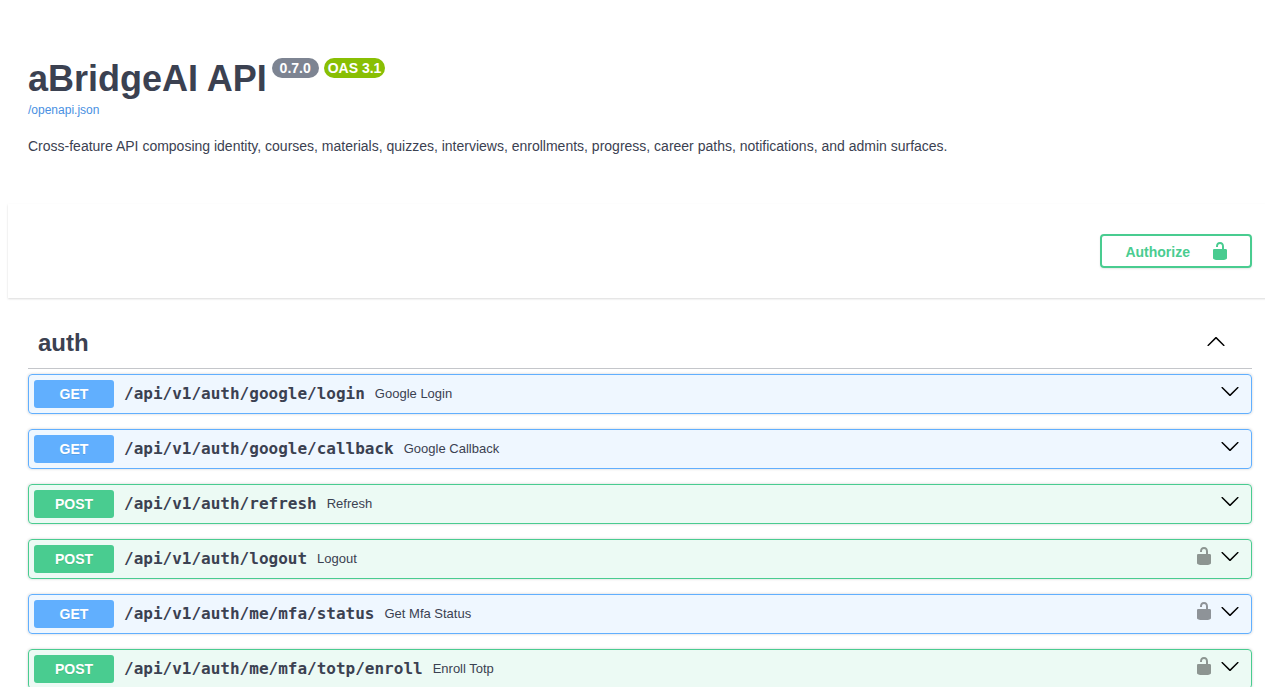
\includegraphics[width=0.92\textwidth,height=0.82\textheight,keepaspectratio]{graphics/swagger/00_overview.png}
    \caption{Live Swagger UI at \texttt{/docs} (rendered from the FastAPI \texttt{/openapi.json}): title, authorise control, and the \texttt{auth} audience-tag section.}
    \label{fig:swagger_overview_main}
\end{figure}

% ────────────────────────────────────────────────────────────
\subsubsection{Authentication Strategy}
% ────────────────────────────────────────────────────────────

The platform offers a single sign-in path: Google SSO. Username/password, password-reset, and email-verification endpoints intentionally do not exist --- this eliminates an entire class of credential-related bugs and shifts identity-proofing to Google's hardened identity provider.

The application issues an access/refresh token pair as the canonical authentication primitive. The \textbf{access token} is a stateless HS256-signed JWT carrying \path|sub| (user ID), \path|sid| (session ID), \path|iat|, and \path|exp|; it is the only credential validated on every API request. The \textbf{refresh token} is a high-entropy opaque random string returned to the client once on login and rotated on every refresh. The two tokens have very different storage profiles, summarised in Table~\ref{tab:auth_tokens_main}.

\begin{longtable}{|p{0.16\textwidth}|p{0.27\textwidth}|p{0.12\textwidth}|p{0.32\textwidth}|}
    \caption{Token pair issued on successful Google login --- backend storage.} \label{tab:auth_tokens_main} \\
    \hline
    \textbf{Token} & \textbf{Purpose} & \textbf{Lifetime} & \textbf{Backend storage} \\
    \hline
    \endfirsthead
    \multicolumn{4}{c}{\small\tablename~\thetable{} \textit{(continued)}} \\
    \hline
    \textbf{Token} & \textbf{Purpose} & \textbf{Lifetime} & \textbf{Backend storage} \\
    \hline
    \endhead
    \hline
    \endfoot
    \path|access_token|  & Authenticates every API request via \path|Authorization: Bearer| & 15 minutes & Stateless JWT, never persisted; validated against \path|auth_sessions| via the embedded \path|sid| claim. \\
    \hline
    \path|refresh_token| & Rotates the access/refresh pair via \path|POST /auth/refresh|     & 7 days     & Raw token returned to client once; only the SHA-256 hash is persisted in \path|auth_sessions.refresh_token_hash|. Rotated on every refresh. \\
    \hline
\end{longtable}

\paragraph{Hot-path session cache.} On every authenticated request the backend must verify that the JWT's \path|sid| still references a live, non-revoked, MFA-cleared session. To keep this check off the database, session state is cached in Redis under \path|session:{session_id}| with a 60-second TTL. A reverse-index Redis \path|SET| at \path|user_sessions:{user_id}| stores all active session IDs for a user, enabling \path{O(N)} cascade revocation when an administrator disables an account (without an unsafe \path|SCAN MATCH session:*|). The cache is read-through with safe fallback: any Redis error logs a warning and the request transparently falls through to PostgreSQL, so a Redis outage degrades latency rather than availability.

\paragraph{Login flow.} \path|GET /auth/google/login| returns an authorisation URL plus an opaque \path|state|; the SPA stores \path|state| and redirects the browser to Google. Google redirects back with a \path|code|; the SPA forwards it to \path|GET /auth/google/callback|, which exchanges the code with Google, finds (or rejects) the application user --- the platform requires the email to match a pre-provisioned account; self-signup is not supported --- and returns the token pair plus a \path|requires_mfa| flag. If \path|requires_mfa| is \path|true|, the SPA navigates to the MFA challenge screen and exchanges the pre-MFA token for an MFA-completed token via the challenge / verify pair.

\paragraph{MFA.} TOTP-based MFA is exposed as a self-service feature under \path|/auth/me/mfa|. Once enrolled, every fresh login produces a pre-MFA token; \path|POST .../challenge| opens a challenge and \path|POST .../verify| accepts either a TOTP code or a single-use recovery code. Sensitive operations (regenerating recovery codes, disabling MFA) require an inline proof-of-possession check so a stolen access token cannot silently turn off the second factor. The complete MFA endpoint list is in Appendix~\ref{appendix:api-design}.

% ────────────────────────────────────────────────────────────
\subsubsection{Error Handling}
% ────────────────────────────────────────────────────────────

Errors surface as standard FastAPI \path|HTTPException| responses with a JSON body of \path|{detail: ...}| and a numeric status code. The application defines a small hierarchy of exceptions (\path|AppError|, \path|NotFoundError|, \path|UnauthorizedError|, \path|ForbiddenError|, \path|ConflictError|) raised by the service layer and translated to HTTP at the router boundary. For richer cases (OAuth provisioning, MFA gates, validation failures) the \path|detail| is an object that carries a stable \path|error| code so the SPA can branch deterministically:

\begin{verbatim}
HTTP/1.1 403 Forbidden
Content-Type: application/json

{
  "detail": {
    "error": "oauth_account_not_provisioned",
    "message": "This Google account is not linked to a registered user."
  }
}
\end{verbatim}

The full status-code map (200, 201, 202, 204, 400, 401, 403, 404, 409, 422, 503) and the corresponding exception types are tabulated in Appendix~\ref{appendix:api-design}.

% ────────────────────────────────────────────────────────────
\subsubsection{Endpoint Surface (overview)}
% ───────────────────────────────────────────────────────────

The 195 routes mounted under \path|/api/v1| are partitioned across 12 features. Table~\ref{tab:api_features_main} summarises the feature breakdown; per-route specifications are catalogued in Appendix~\ref{appendix:api-design}.

\begin{longtable}{|p{0.22\textwidth}|p{0.1\textwidth}|p{0.56\textwidth}|}
    \caption{Feature breakdown of the API surface.} \label{tab:api_features_main} \\
    \hline
    \textbf{Feature} & \textbf{Routes} & \textbf{Audience routers} \\
    \hline
    \endfirsthead
    \multicolumn{3}{c}{\small\tablename~\thetable{} \textit{(continued)}} \\
    \hline
    \textbf{Feature} & \textbf{Routes} & \textbf{Audience routers} \\
    \hline
    \endhead
    \hline
    \endfoot
    Identity         & 16 & \path|auth|, \path|me|, \path|users|, \path|mfa| \\ \hline
    Access control   & 26 & \path|admin|, \path|organizations| \\ \hline
    Courses          & 48 & \path|learner| (\path|/me/courses|), \path|authoring| (\path|/teacher|), \path|assignment| (\path|/dept|), \path|administration| (\path|/admin|) \\ \hline
    Materials        & 17 & \path|authoring| (\path|/teacher|), \path|learner| (\path|/materials|) \\ \hline
    Quizzes          & 22 & \path|authoring| (\path|/teacher|), \path|learner| \\ \hline
    Interviews       & 21 & \path|authoring| (\path|/teacher|), \path|learner| \\ \hline
    Progress         &  7 & \path|learner| (\path|/me/progress|), \path|authoring| (\path|/teacher|) \\ \hline
    Career paths     &  2 & \path|learner| \\ \hline
    Spaced repetition&  7 & \path|learner| (\path|/me|), \path|teacher| \\ \hline
    Notifications    &  7 & \path|learner| (\path|/me/notifications|) \\ \hline
    Admin operations & 19 & \path|stats|, \path|users|, \path|processing|, \path|ai_costs|, \path|audit| \\ \hline
    Health           &  3 & root and \path|/api/v1| (K8s probes + SPA reach) \\ \hline
\end{longtable}

% ────────────────────────────────────────────────────────────
\subsubsection{Pagination, Filtering and Idempotency}
% ────────────────────────────────────────────────────────────

\paragraph{Pagination.} Every list endpoint uses cursor pagination via the generic \path|CursorPage[T]| dataclass at \path|core/pagination/cursor.py|. The response envelope is \verb*~{items: T[], next_cursor: string | null}~; the cursor is a base64-encoded UUID (or ISO-8601 timestamp for time-ordered feeds) of the last row returned, opaque to the client. Clients pass it back as \path|?cursor=...| paired with an optional \path|limit| (default 20, max 100); \path|next_cursor| being \path|null| signals end-of-list. The scheme keeps queries on a single index column, avoids the \path{O(N)} skip cost of \path|OFFSET| on deep pages, and tolerates inserts/deletes between fetches without duplicating or skipping rows.

\paragraph{Filtering and sorting.} List endpoints accept feature-specific filters as query parameters (e.g.\ \path|status=published|, \path|role=teacher|, \path|q=<search>|). Sort order is fixed per endpoint and documented inline; freeform sort keys are deliberately not supported to keep the index strategy predictable.

\paragraph{Idempotency.} Mutating endpoints that may be retried by the SPA (in particular \path|POST .../attempts| during quiz submission and the bulk \path|POST .../quizzes/{id}/generate|) accept an optional \path|Idempotency-Key| header; the backend deduplicates against this key for a 24-hour window. AI generation endpoints additionally return an \path|Operation-Location| header pointing to \path|.../generation-runs/{run_id}| for progress polling.

% ────────────────────────────────────────────────────────────
\subsubsection{API Design Summary}
% ────────────────────────────────────────────────────────────

\begin{longtable}{|p{0.22\textwidth}|p{0.30\textwidth}|p{0.36\textwidth}|}
    \caption{API design summary --- strategies and rationale.} \label{tab:api_summary_main} \\
    \hline
    \textbf{Concern} & \textbf{Strategy} & \textbf{Rationale} \\
    \hline
    \endfirsthead
    \multicolumn{3}{c}{\small\tablename~\thetable{} \textit{(continued)}} \\
    \hline
    \textbf{Concern} & \textbf{Strategy} & \textbf{Rationale} \\
    \hline
    \endhead
    \hline
    \endfoot
    Architecture     & Vertical-slice features; routers $\to$ services $\to$ queries & Feature ownership; CI-enforced layering boundary. \\ \hline
    Authentication   & Google OAuth $\to$ JWT bearer pair (access + refresh)        & No password surface; identity proofing delegated to Google. \\ \hline
    MFA              & TOTP + recovery codes; pre-MFA gate on the access token      & Stolen access tokens cannot act before MFA. \\ \hline
    Authorisation    & Role-scoped URL prefix + per-route dependency check          & Clear contextual boundary; central dependency for permission lookups. \\ \hline
    Versioning       & URL path \path|/api/v1|                                      & Explicit, easy to migrate via a co-existing v2 prefix later. \\ \hline
    Error format     & FastAPI \path|HTTPException| with structured \path|detail|   & Standard, well-supported in OpenAPI tooling and the SPA's error layer. \\ \hline
    Pagination       & Cursor (\path|next_cursor|) uniformly across every list endpoint & Stable deep traversal; constant cost per page; no row duplication under concurrent writes. \\ \hline
    Idempotency      & Optional \path|Idempotency-Key| header (24-hour window)      & Safe SPA retries on quiz submission and AI generation. \\ \hline
    Long-running AI  & Async dispatch via ARQ + \path|generation-runs/{run_id}|     & HTTP layer stays under hundreds of milliseconds; progress is observable. \\ \hline
    Object storage   & S3-compatible (Garage); presigned multipart uploads          & Browser uploads bypass the application server. \\ \hline
    Observability    & \path|http_audit_log| middleware + \path|admin/audit/*|      & Per-request trace surface. \\ \hline
\end{longtable}
